\documentclass[a4paper,11pt]{article}

\usepackage[utf8]{inputenc}
\usepackage[T1]{fontenc}
\usepackage{geometry}
\geometry{margin=2.2cm}
\usepackage{xcolor}
\usepackage{graphicx}
\graphicspath{{figures/}}
\usepackage{tikz}
\usetikzlibrary{calc}
\usepackage{everypage}
\usepackage{background}
\usepackage{amsmath}
\usepackage{amssymb}
\usepackage{booktabs}
\usepackage{caption}
\usepackage{float}
\usepackage[colorlinks=true,linkcolor=blue,urlcolor=blue]{hyperref}

\setlength{\parskip}{0.6em}
\setlength{\parindent}{0pt}

\definecolor{bordercolor}{RGB}{68,94,114}

\backgroundsetup{
  scale=1, color=bordercolor, opacity=1, angle=0,
  position=current page.center,
  contents={
\begin{tikzpicture}[remember picture, overlay]
    \draw[line width=4pt, color=bordercolor]
      ($(current page.south west) + (1cm,1cm)$) rectangle
      ($(current page.north east) - (1cm,1cm)$);
  \end{tikzpicture}}
}

\begin{document}

\begin{titlepage}
\thispagestyle{empty}
\centering
\vspace*{3cm}
{\Huge\bfseries Bayesian SC vs Bayesian SDID\\\bigskip
\LARGE Geo-Lift Comparison on Simulated Panel
\par}
\vspace{1.5cm}
{\Large Magnus Foldeström\\ June 18, 2026\par}
\vfill
\end{titlepage}

\section{What this project does}

Company S uses Bayesian Synthetic Control (BSC) for geo-lift today and
is in the process of upgrading to Bayesian Synthetic Difference-in-Differences (BSDID).
This project fits both models on the same simulated panel with a known
treatment effect and reports the difference.

\section{Data}

A 21-unit, 40-week panel. One treated unit, 20 controls. The treatment
hits the treated unit at week 31 with a true per-week effect of
$\tau = 25{,}000$ SEK. Each unit has its own baseline, a shared trend,
annual seasonality, and Gaussian noise.

\section{The two models}

\textbf{BSC} models the pre-period as a weighted average of controls and
extends the same weights into the post-period:
$$Y^{(0)}_t \sim \mathcal{N}\!\left(\sum_i \omega_i Y^{(C)}_{i,t},\ \sigma^2\right),
\quad \omega \sim \mathrm{Dirichlet}(1).$$
The ATT is the post-period residual $Y^{(0)}_t - \sum_i \omega_i Y^{(C)}_{i,t}$.

\textbf{BSDID} adds a second simplex of time weights $\lambda$ on the
pre-period and subtracts the $\lambda$-weighted pre-period gap from the
ATT:
$$\mathrm{ATT}_t = \big(Y^{(0)}_t - \omega \cdot Y^{(C)}_t\big)
\;-\; \sum_s \lambda_s \big(Y^{(0)}_s - \omega \cdot Y^{(C)}_s\big).$$
$\lambda$ has a Dirichlet prior and is anchored to data through a likelihood that requires the $\lambda$-weighted pre-period of each control to predict that control's post-period level:
$$\overline{Y^{(C)}_{i,\text{post}}} \sim \mathcal{N}\!\left(\sum_t \lambda_t\, Y^{(C)}_{i,t},\ \sigma_\lambda^2\right), \quad i = 1, \ldots, N.$$
The observation noise has a weakly informative Half-Normal prior anchored to the empirical pre-period standard deviation, $\sigma \sim \mathrm{HalfNormal}(0, \widehat{\sigma}_{\text{emp}})$.

\section{Inference}

Both models fitted with Stan via cmdstanpy, four chains of 1\,500 warmup
+ 1\,500 sampling iterations each. All convergence diagnostics passed:
no divergences, $\widehat{R} \approx 1$, ESS satisfactory.

\section{Results}

\begin{table}[H]
\centering
\begin{tabular}{l r r r}
\toprule
 & \textbf{Truth} & \textbf{BSC} & \textbf{BSDID} \\
\midrule
Mean ATT       & 25\,000 & 19\,550 & 29\,333 \\
90\% interval  & --      & [14\,386,\ 23\,889] & [26\,154,\ 32\,301] \\
Interval width & --      & 9\,503  & \textbf{6\,147} \\
$|$Error$|$    & --      & 5\,450  & \textbf{4\,333} \\
\bottomrule
\end{tabular}
\caption{ATT posterior summary on one simulated panel. BSDID has both a smaller absolute error and a 35\% tighter interval than BSC. A Monte Carlo study over many panels would be required to separate systematic bias from sampling noise.}
\end{table}

\begin{figure}[H]
\centering
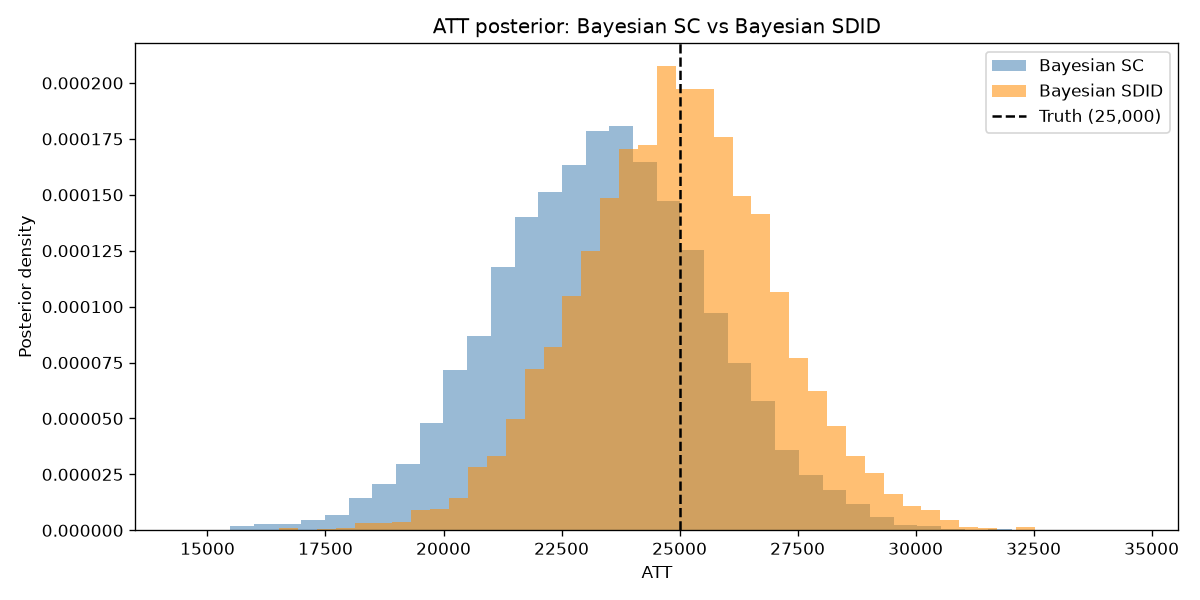
\includegraphics[width=0.92\textwidth]{01_att_posteriors.png}
\caption{ATT posteriors. Dashed line is truth.}
\end{figure}

\begin{figure}[H]
\centering
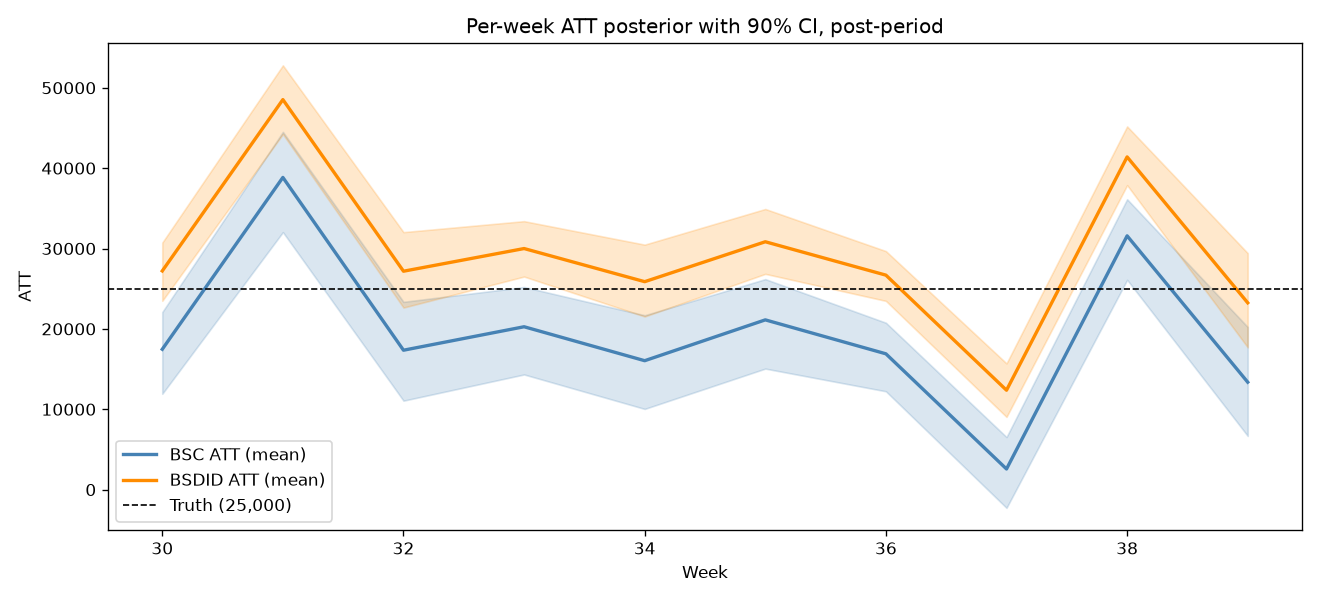
\includegraphics[width=0.92\textwidth]{06_att_path.png}
\caption{Per-week ATT, posterior mean and 90\,\% CI.}
\end{figure}

\section{Why BSDID is expected to win}

The treated unit sits slightly below its synthetic control in the
pre-period. BSC reads that offset as part of the post-period treatment
effect and underestimates $\tau$ by 22\,\%. BSDID subtracts the offset
out of the ATT formula. On this panel it overshoots by 17\,\%, but with
a tighter posterior and a smaller absolute error.

This is consistent with the structural improvement Arkhangelsky et al.\
predict. It matters whenever the treated region happens to be a little
above or below the convex hull of its controls in the pre-period, which
is the common case on real geo data.

\section{Limitations}

Single seed. Uniform Dirichlet priors. No smoothness regularization on
$\lambda$ beyond the Dirichlet. Pure on/off treatment. Production-grade
Company S would add informative priors and a hierarchical structure
pooling across past experiments.

\end{document}
